% !TEX TS-program = XeLaTeX
% use the following command:
% all document files must be coded in UTF-8
\documentclass[portuguese]{textolivre}
% build HTML with: make4ht -e build.lua -c textolivre.cfg -x -u article "fn-in,svg,pic-align"

\journalname{Texto Livre}
\thevolume{15}
%\thenumber{1} % old template
\theyear{2022}
\receiveddate{\DTMdisplaydate{2021}{8}{6}{-1}} % YYYY MM DD
\accepteddate{\DTMdisplaydate{2021}{10}{6}{-1}}
\publisheddate{\DTMdisplaydate{2021}{11}{9}{-1}}
\corrauthor{Vinicius Carvalho Pereira}
\articledoi{10.35699/1983-3652.2022.35555}
%\articleid{NNNN} % if the article ID is not the last 5 numbers of its DOI, provide it using \articleid{} commmand
\runningauthor{Silveira e Pereira} 
%\editorname{Leonardo Araújo} % old template
\sectioneditorname{Daniervelin Pereira}
\layouteditorname{Anna Izabella Pereira}

\title{As imagens do duplo e da mão na obra digital hipertextual \emph{88 Constellations for Wittgenstein (to Be Played with the Left Hand)}, de David Clark}
\othertitle{The images of the double and the hand in the digital hypertextual work 88 Constellations for Wittgenstein (to Be Played with the Left Hand), by David Clark}
% if there is a third language title, add here:
%\othertitle{Artikelvorlage zur Einreichung beim Texto Livre Journal}

\author[1]{Alice Garcia da Silveira \orcid{0000-0002-5938-0963} \thanks{Email: \url{alice.garcia.silveira@gmail.com}}}
\author[2]{Vinícius Carvalho Pereira \orcid{0000-0003-1844-8084} \thanks{Email: \url{viniciuscarpe@gmail.com}}}
\affil[1]{Secretaria de Estado de Educação de Mato Grosso, Cuiabá, MT, Brasil.}
\affil[2]{Universidade Federal de Mato Grosso, Departamento de Letras, Cuiabá, MT, Brasil.}

\addbibresource{article.bib}
% use biber instead of bibtex
% $ biber article

% used to create dummy text for the template file
\definecolor{dark-gray}{gray}{0.35} % color used to display dummy texts
\usepackage{lipsum}
\SetLipsumParListSurrounders{\colorlet{oldcolor}{.}\color{dark-gray}}{\color{oldcolor}}

% used here only to provide the XeLaTeX and BibTeX logos
\usepackage{hologo}

% if you use multirows in a table, include the multirow package
\usepackage{multirow}

% provides sidewaysfigure environment
\usepackage{rotating}

% CUSTOM EPIGRAPH - BEGIN 
%%% https://tex.stackexchange.com/questions/193178/specific-epigraph-style
\usepackage{epigraph}
\renewcommand\textflush{flushright}
\makeatletter
\newlength\epitextskip
\pretocmd{\@epitext}{\em}{}{}
\apptocmd{\@epitext}{\em}{}{}
\patchcmd{\epigraph}{\@epitext{#1}\\}{\@epitext{#1}\\[\epitextskip]}{}{}
\makeatother
\setlength\epigraphrule{0pt}
\setlength\epitextskip{0.5ex}
\setlength\epigraphwidth{.7\textwidth}
% CUSTOM EPIGRAPH - END

% LANGUAGE - BEGIN
% ARABIC
% for languages that use special fonts, you must provide the typeface that will be used
% \setotherlanguage{arabic}
% \newfontfamily\arabicfont[Script=Arabic]{Amiri}
% \newfontfamily\arabicfontsf[Script=Arabic]{Amiri}
% \newfontfamily\arabicfonttt[Script=Arabic]{Amiri}
%
% in the article, to add arabic text use: \textlang{arabic}{ ... }
%
% RUSSIAN
% for russian text we also need to define fonts with support for Cyrillic script
% \usepackage{fontspec}
% \setotherlanguage{russian}
% \newfontfamily\cyrillicfont{Times New Roman}
% \newfontfamily\cyrillicfontsf{Times New Roman}[Script=Cyrillic]
% \newfontfamily\cyrillicfonttt{Times New Roman}[Script=Cyrillic]
%
% in the text use \begin{russian} ... \end{russian}
% LANGUAGE - END

% EMOJIS - BEGIN
% to use emoticons in your manuscript
% https://stackoverflow.com/questions/190145/how-to-insert-emoticons-in-latex/57076064
% using font Symbola, which has full support
% the font may be downloaded at:
% https://dn-works.com/ufas/
% add to preamble:
% \newfontfamily\Symbola{Symbola}
% in the text use:
% {\Symbola }
% EMOJIS - END

% LABEL REFERENCE TO DESCRIPTIVE LIST - BEGIN
% reference itens in a descriptive list using their labels instead of numbers
% insert the code below in the preambule:
%\makeatletter
%\let\orgdescriptionlabel\descriptionlabel
%\renewcommand*{\descriptionlabel}[1]{%
%  \let\orglabel\label
%  \let\label\@gobble
%  \phantomsection
%  \edef\@currentlabel{#1\unskip}%
%  \let\label\orglabel
%  \orgdescriptionlabel{#1}%
%}
%\makeatother
%
% in your document, use as illustraded here:
%\begin{description}
%  \item[first\label{itm1}] this is only an example;
%  % ...  add more items
%\end{description}
% LABEL REFERENCE TO DESCRIPTIVE LIST - END


% add line numbers for submission
%\usepackage{lineno}
%\linenumbers

\begin{document}
\maketitle

\begin{polyabstract}
\begin{abstract}
O presente artigo visa analisar os percursos temáticos em torno das imagens do duplo e da mão dentro da obra digital hipermídia \emph{88 Constellations for Wittgenstein (to Be Played with the Left Hand)}, do artista canadense David Clark \cite*{clark2010}. Para tanto, o artigo inicialmente procede à apresentação panorâmica do campo da literatura digital e de algumas questões terminológicas da área. Na sequência, apresenta-se uma descrição detalhada da estrutura e do funcionamento do \textit{corpus}, bem como sua inserção no cânone da literatura eletrônica, antes de passar à análise propriamente dita dos percursos temáticos selecionados. As discussões empreendidas no artigo, por meio de \textit{close reading} hipertextual, evidenciam a riqueza dessa obra digital e multimodal, que poderia ser lida em variados percursos interpretativos, dos quais destacamos duas rotas interpretativas construídas com base em recorrências temáticas entre fragmentos interconectados sobre vida e obra do filósofo austro-britânico Ludwig Wittgenstein. Além disso, o artigo reflete sobre os desafios para interpretação de uma obra hipertextual digital, ressaltando a importância das escolhas metodológicas para a análise de um objeto cultural com tais especificidades midiáticas e semióticas.

\keywords{Ciberliteratura \sep Hipertextualidade \sep Percursos de leitura \sep Duplo \sep Mão}
\end{abstract}

\begin{english}
\begin{abstract}
This paper aims to analyze the possible thematic routes of the images of the double and the hand in the digital hypermedia work \emph{88 Constellations for Wittgenstein (to Be Played with the Left Hand)}, by Canadian artist David Clark \cite*{clark2010}. To do so, we initially present an overview of the field of digital literature and some of its main terminological issues. Subsequently, we describe in detail the structure and functions of the corpus, as well as its place within the canon of electronic literature, before we in fact analyze the selected thematic routes. By means of hypertextual close reading, the discussions in the article show the richness of this digital and multimodal work, which could be read according to various interpretive paths, from which we highlight two interpretative routes built on thematic recurrences among interconnected fragments about the life and work of Austrian-British philosopher Ludwig Wittgenstein. Moreover, this article reflects on the challenges to interpreting digital hypertextual works as this one, highlighting the methodological choices inherent to the analysis of a cultural object with such mediatic and semiotic specificities.

\keywords{Cyberliterature \sep Hypertextuality \sep Reading routes \sep Double \sep Hand}
\end{abstract}
\end{english}
% if there is another abstract, insert it here using the same scheme
\end{polyabstract}

\section{Introdução}\label{sec-intro}
Este artigo visa analisar os percursos temáticos em torno das imagens do duplo e da mão, selecionadas dentro de um universo maior, composto pela totalidade das rotas de leitura possíveis dentro da obra de literatura digital \emph{88 Constellations for Wittgenstein (to Be Played with the Left Hand)}, de David \textcite{clark2010}. A partir da análise dessas rotas, propõe-se que a recorrência temática pode ser um elemento produtivo na construção de uma interpretação coerente dos fragmentos interconectados por hiperlinks. Para tanto, procedemos inicialmente a uma apresentação panorâmica do campo da literatura digital antes da análise do corpus propriamente dito. 

Com o advento de novas tecnologias e a consolidação da era digital, surge uma nova forma de experimentos com literatura, a ciberliteratura, também intitulada literatura eletrônica ou literatura digital. A \emph{Electronic Literature Organization} (ELO), maior organização internacional dedicada aos estudos ciberliterários, define que uma obra de literatura eletrônica é aquela que contém “um aspecto literário importante que aproveita as capacidades e contextos fornecidos por um computador independente ou em rede” \cite[p. 21]{hayles2009}.

“Ciberliteratura” é o termo utilizado por Lúcia \textcite{santaella2012}, importante pesquisadora brasileira dessa esfera cultural, para se referir à literatura digital-born, isto é, aquela que foi concebida para o meio digital. Dessa forma, obras físicas que foram posteriormente digitalizadas não se enquadrariam na definição da estudiosa, como no caso das obras completas de Machado de Assis, digitalizadas e disponíveis na Web.

Já o termo “literatura digital” é usado mais frequentemente por pesquisadores da América Latina, como Carolina \textcite[p. 4]{gainza2013}, que se refere “àquela literatura concebida em um formato digital para ser lida na tela de um dispositivo eletrônico interativo”. A autora também reforça que se trata de uma literatura não transponível para o analógico, dado que se vale de características específicas do digital, como a manipulabilidade e a modularidade dos dados.

Embora reconheçamos que cada um desses termos designa o campo a partir de uma perspectiva (da eletroeletrônica, da cibernética ou dos dispositivos não analógicos), seu uso é frequentemente intercambiável, designando, de modo geral, produções literárias desenvolvidas nas novas mídias, especialmente para/em/com dispositivos computacionais.

É importante destacar que, ao tratarmos de formas ciberliterárias, referimo-nos a textos que vão além dos códigos verbais e não verbais exibidos na tela: valem-se também de códigos computacionais, de bancos de dados, de recursos de \emph{hardware} e da interconectividade cara às redes digitais. Nesse sentido, observamos experimentações tanto na interface entre arte e tecnologia, que se popularizou no Brasil mais rapidamente no campo das Artes Visuais, quanto de iniciativas no âmbito da hibridização contemporânea da literatura com outras mídias. Tais projetos são indicativos de uma tendência maior da literatura contemporânea, “que enfatiza o transbordamento de alguns dos limites mais conspícuos que haviam definido o literário com relativa comodidade, pelo menos até os anos sessenta” \cite[p. 1]{garramuno2009}. Justamente da década de sessenta do século XX, marco temporal apontado por Garramuño para a explosão da literatura como campo expansivo e inespecífico, datam as primeiras experimentações com arte digital e literatura digital, num longo processo que culminaria, anos mais tarde, na composição de obras em formatos inovadores, como romances hipertextuais eletrônicos.

Cabe ressaltar que autores como \textcite{rettberg2019, funkhouser2012} citam algumas modalidades importantes de literatura eletrônica, a saber: a hipertextual, com estrutura não linear, formada por blocos de texto (lexias) que se conectam por links eletrônicos; a generativa, que consiste em processos (semi)automáticos de produção de textos por meio da combinatória de dados; e a hipermídia, que associa elementos multimodais estáticos e dinâmicos. Muitas obras, contudo, perpassam diferentes gêneros, dado que reúnem características muito variadas, todas processáveis em códigos binários.

Nesta introdução foram apresentados, em linhas gerais, os conceitos de ciberliteratura e seus correlatos, bem como indicadas algumas de suas modalidades, que podem ser realizadas em diferentes gêneros, como romances hipertextuais, poemas generativos, contos hipermídia etc. As próximas seções tratam da obra ciberliterária analisada neste trabalho, \emph{88 Constellations for Wittgenstein (to Be Played with the Left Hand)}, de David Clark, uma peça que combina recursos hipertextuais e hipermidiáticos com fins tanto narrativos quanto especulativos acerca da vida e obra de Ludwig Wittgenstein.

A fusão de diferentes tipologias textuais e de diferentes recursos computacionais na composição de \emph{88 Constellations} está em íntima relação com importantes paradigmas dos estudos literários contemporâneos, os quais ressaltam o caráter onívoro do romance \cite{perrone-moises2016} – e, portanto, sua inespecificidade \cite{garramuno2014} –, reforçada pela convergência de diferentes mídias, que marca um novo paradigma cultural no qual se observam “três conceitos – convergência dos meios de comunicação, cultura participativa e inteligência coletiva”. \cite[p. 29]{jenkins2009}. Como obra hipermidiática e hipertextual, em que o leitor tem papel ativo ao interagir com a interface para definir seu próprio percurso pelo texto e constituir, \emph{88 Constellations} está em pleno acordo com paradigmas da hibridação, da inespecificidade, da convergência – caros, aliás, a boa parte da produção de literatura digital.

Diante da riqueza da obra, por nós tomada como um romance hipermidiático e hipertextual, faremos sua apresentação geral antes de avançarmos para a leitura dos percursos temáticos do duplo e da mão. Reforçamos ainda a importância dessa apresentação diante do desafio que hoje se coloca a um potencial leitor de \emph{88 Constellations}: a obra foi desenvolvida para a plataforma \emph{Flash} (que permitiu a ciberartistas por quase trinta anos a criação de animações digitais com relativa facilidade), mas tal tecnologia foi descontinuada pela empresa Adobe no final de 2020. Assim, o trabalho de Clark só pode hoje ser parcialmente revisitado, seja por recurso a programas emuladores (que simulam o funcionamento do \emph{Flash Player}), seja pela documentação e descrição das interfaces\footnote{Como a seção 2 do trabalho inclui a apresentação de uma obra não mais executável nos navegadores de Internet mais populares, ela retoma partes da contextualização publicada em SILVEIRA, Alice Garcia; PEREIRA, Vinícius Carvalho. \emph{88 Constellations for Wittgenstein (to Be Played with the Left Hand)}, de David Clark: análise de um percurso temático por seus hiperlinks. In: MOREIRA, Maria Elisa Rodrigues; PEREIRA, Vinícius Carvalho; FIORINI, Juan Ferreira. Palavra e imagem em deslocamento. Belo Horizonte: Tradição Planalto, 2020. Ressalte-se, porém, o ineditismo da análise dos percursos temáticos do duplo e da mão em \emph{88 Constellations}, foco do presente artigo.}, como procedemos a seguir.

Cumpre ainda ressaltar que procedemos neste artigo a uma leitura da obra centrada nas técnicas de \emph{close reading}. Se essa é uma metodologia já bastante comum nos estudos literários, com suas potencialidades e limitações referenciadas em muitas publicações no âmbito da Teoria Literária, os ganhos de uma análise imanente do texto são ampliados quando se trata de uma obra como \emph{88 Constellations}, dado que sua descrição serve não apenas a fins críticos, senão também de documentação da obra, não mais executável em navegadores populares de Internet. Ademais, em se tratando de um campo literário em formação, a literatura digital pode se beneficiar de análises centradas em sua materialidade na medida em que estas ajudam a balizar pontos de interesse crítico a serem observados em outras obras do gênero. 

\section{As 88 constelações de Clark: o percurso do duplo}
\emph{88 Constellations for Wittgenstein (to Be Played with the Left Hand)} é uma obra hipertextual e hipermidiática ciberliterária do canadense David \textcite{clark2010} que foi incluída no terceiro volume da \emph{Electronic Literature Collection}, da Electronic Literature Organization (ELO). A inclusão da obra na referida antologia é um importante ponto para a compreensão de sua importância no cenário da literatura eletrônica, dado que as coletâneas publicadas a cada cinco anos (vol.1 – 2006, vol.2 – 2011, vol.3 – 2016 e vol.4 – 2021, no prelo) pela ELO figuram entre os mais importantes dispositivos de canonização no campo ciberliterário.

Assim a ELO define a obra:

\begin{quote}
    Projetado com requinte, com um vocabulário visual confiante e discreto, baseado em ícones e imagens degradadas, 88 Constellations às vezes pode parecer um documentário independente bem elaborado, mas que se desvia de reportagens biográficas aparentemente normativas para trocadilhos visuais, associações fantásticas e digressões peculiares. Infundido com o paradoxo, ludicidade e paranoia ocasional da vida do filósofo, este é um trabalho massivo com uma lógica de círculos dentro de círculos que levaria várias horas para esgotar. Como os New Digital Emblems de William Poundstone, 88 Constellations é uma obra-prima multimídia interativa sobre o lúdico que amplia as atividades de seu suposto tema como "um biscoito da sorte filosófico". \cite[n. p., tradução nossa]{electronic2010}\footnote{No original: \emph{Exquisitely designed with a confident, understated visual vocabulary relying on icons and degraded images, 88 Constellations at times can feel like a really well-made independent documentary, but one which swerves from seemingly normative biographical reportage into visual puns, fantastic associations, and quirky digressions. Infused with the paradox, playfulness and occasional paranoia of the philosopher's life, this is a massive work with circles-within-circles logic that would take several hours to exhaust. Like William Poundstone's New Digital Emblems, 88 Constellations is a tour-de-force interactive, multimedia essay about the ludic that extends the activities of its purported subject like "a philosophical fortune cookie}.}.
\end{quote}

\emph{88 Constellations} tem como tema central o filósofo austro-britânico Ludwig Wittgenstein e trata das relações que fatos de sua vida e obra estabelecem com outros de naturezas distintas, nem sempre óbvios, mas arquitetados com a função de relacioná-los, de alguma forma, à figura do filósofo. Na \emph{homepage} da obra (\Cref{fig1}), pode-se ter acesso a alguns links à disposição do leitor (ou jogador, como sugere o verbo “play” no título): o Enter, que dá acesso à obra; o link Blog, que leva a uma página paratextual metalinguística dedicada a \emph{88 Constellations}, em que podemos encontrar textos do autor, como a descrição da obra, informações sobre Clark, menções, premiações e links para outros trabalhos do autor ou de colegas; \emph{Chemical Pictures}, portfólio de David Clark; e \emph{A is for Apple}, um link com acesso direto a uma de suas obras mais conhecidas e que apresenta características similares às de \emph{88 Constellations}, como hipertextualidade, uso da plataforma \emph{Adobe Flash}, música, imagens fragmentadas e instanciação do papel ativo do leitor na construção da narrativa. 

\begin{figure}[htbp]
 \centering
 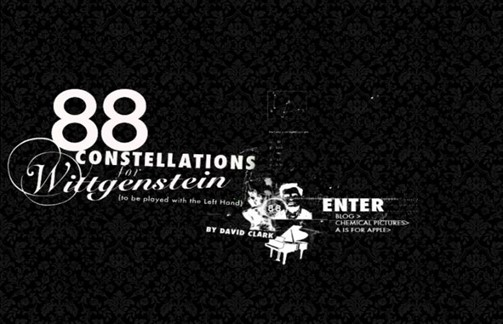
\includegraphics[width=0.5\textwidth]{Fig1[1].jpg}
 \caption{Página inicial do site de \emph{88 Constellations}.}
 \label{fig1}
 \source{\url{ http://www.88constellations.net/88.html}.}
\end{figure}

Ao clicar na logo da obra ou no link Enter, pode-se ouvir a seguinte introdução, acompanhada de imagens animadas, sons e representações de constelações: 

\begin{quote}
Ligue os pontos, faça imagens no céu. Conecte o emaranhado do nosso pensamento a esses desenhos no céu. Esta história é sobre um homem chamado Wittgenstein. Ele era filósofo. Sua vida foi uma série de momentos, e nossa história é uma série de constelações. \cite[n. p., tradução nossa]{clark2010}\footnote{No original: Join the dots together; make pictures in the sky. Connect the muddle of our thinking to these drawings in the sky. This story is about a man named Wittgenstein. He was a philosopher. His life was a series of moments, and our story is a series of constellations.}.
\end{quote}

Por meio da imagem do jogo infantil de “ligar os pontos”, a descrição conecta a estrutura hipertextual, a metáfora das constelações e o pivô da obra – o filósofo Wittgenstein. No canto da página, há o link \emph{Skip}, que pula a introdução se o leitor assim quiser. Depois da introdução, um mapa das 88 constelações conhecidas atualmente pela Astronomia é disponibilizado, e ele traz o número 8 na posição horizontal, em possível referência ao símbolo do infinito, tema bastante presente nos estudos do filósofo, além de sinalizar que, em contexto literário – e, em muitos casos, de forma acentuada em obras ciberliterárias –, os limites das obras são imprecisos, possibilitando um sem-fim de leituras diferentes, de acordo com as escolhas de cada leitor. Nesse sentido, dialoga-se diretamente com o que o próprio David Clark afirma acerca da multiplicidade de sua obra e das possibilidades de leitura:

\begin{quote}
\emph{88 Constellations for Wittgenstein (to be played with the Left Hand)} é uma obra de net.art interativa, não linear, que explora a vida e a filosofia de Ludwig Wittgenstein através de uma série de vinhetas animadas criadas em Flash. Cada uma das 88 seções corresponde a uma das 88 constelações no céu noturno. Cada constelação se torna um dispositivo de navegação para o leitor negociar as relações associativas entre essas vinhetas. Também os leitores podem interagir com cada animação em colagem usando sua mão esquerda para desencadear eventos a partir do teclado do computador (em homenagem ao irmão de Ludwig Wittgenstein, Paul, um pianista de concerto que perdeu seu braço direito na Segunda Guerra Mundial, mas continuou sua carreira tocando obras de piano compostas para a Mão Esquerda). Essa obra considera questões que Ludwig Wittgenstein ponderou em sua carreira como filósofo: lógica, linguagem, a natureza do pensamento e os limites do conhecimento – tudo em relação com nosso mundo digital contemporâneo. \cite[n. p., tradução nossa]{clark2010}\footnote{No original: \emph{88 Constellations for Wittgenstein (to be played with the Left Hand) is an interactive, non-linear net.art piece that explores the life and philosophy of Ludwig Wittgenstein through a series of animated vignettes created in Flash. Each of the 88 sections corresponds to one of the 88 constellations in the night sky. Each constellation becomes a navigation device for the viewer to negotiate the associative relationships between these vignettes. As well, viewers can interact with each collaged animation using their left hand to trigger events from the computer keyboard (in homage to Ludwig Wittgenstein's brother Paul (a concert pianist who lost his right arm in WWI but continued his career performing piano works composed for the Left Hand). This work considers questions that Ludwig Wittgenstein pondered in his career as a philosopher: logic, language, the nature of thinking, and the limits of knowledge -- all in relation to our contemporary digital world.}}.
\end{quote}

Cada constelação de \emph{88 Constellations} é uma lexia da obra, isto é, uma unidade textual conectada a outras por meio de hiperlinks, e cada uma delas é indicada por sua sigla. Durante a leitura desenvolvida nessa pesquisa, observou-se que havia temas recorrentes nas constelações, os quais, naturalmente, relacionavam-se entre si. Após a leitura de cada uma das constelações a partir da lista disponível no \emph{Site Map}, procedeu-se neste trabalho a uma seleção e organização por princípios associativos de acordo com as sequências sugeridas\footnote{Ao selecionar uma constelação na carta celeste que funciona como mapa de navegação na obra, o leitor pode ter acesso a outras constelações próximas, com que geralmente mantêm relações temáticas. Nesse sentido, \emph{88 Constellations for Wittgenstein (to Be Played with the Left Hand)} acaba sugerindo, por expedientes de distribuição especial dos nós da rede (mais próximos ou mais distantes entre si), alguns percursos possíveis ao leitor.} pelo próprio texto, enfocando os temas do duplo e da mão.

Podemos começar a apresentação por diversos pontos, como a constelação \emph{Taurus}, por exemplo, indicada pela sigla TAU. O conteúdo de cada uma dessas lexias pode ser acessado pelo leitor em qualquer ordem ao selecioná-la. Por meio da seleção de qualquer uma dessas constelações, o seu conteúdo, composto por sons cibernéticos, músicas clássicas e populares, imagens, movimentos e interação, é acessado pelo leitor. Alguns desses recursos são disponibilizados a partir do movimento do mouse, enquanto outros são acessados a partir de atalhos no teclado.

\begin{figure}[htbp]
 \centering
 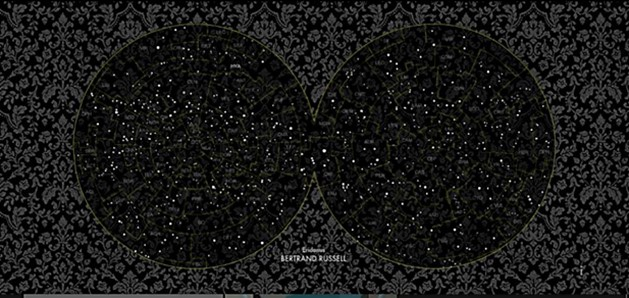
\includegraphics[width=0.6\textwidth]{Fig2[1].jpg}
 \caption{Mapa das constelações.}
 \label{fig2}
 \source{\url{http://www.88constellations.net/88.html}.}
\end{figure}

O número 88 é o tema da constelação 1 de \emph{88 Constellations}, Aquarius (AQU). O narrador mostra as 88 constelações do céu e as 88 teclas do piano; fala sobre os dois infinitos em posição vertical do número 88; apresenta algo em comum entre Wittgenstein, Adolf Hitler e Charles Chaplin, todos nascidos em 1889 (números com os mesmos algarismos nas casas da centena e da dezena), sendo esses os três personagens que podem ser encontrados nas constelações da obra. 

O número 88 é também, nessa constelação, tomado como metáfora visual. \textcite{clark2010} discorre sobre o número que nomeia a constelação: “Oito e oito, oitenta e oito constelações e teclas do piano. Dois infinitos verticais, duas senhoras gordas. 1889: Chaplin, Hitler, Wittgenstein” \cite[n. p., tradução nossa]{clark2010}\footnote{No original: \emph{Eight and eight, eighty-eight Constellations and piano Keys. Two upright infinities, two fat ladies, 1889, Chaplin, Hitler, Wittgenstein}.}. Há indícios, nessa constelação, de algumas das relações que serão traçadas no decorrer de 88 Constellations: a música (\Cref{fig3}); a astronomia (\Cref{fig4}); e a verticalidade, presente na relação entre o símbolo do infinito e o número 8 e em várias referências ao World Trade Center e ao Petronia Towers, dois pares de torres arranha-céus que são mencionados ao longo da obra de Clark. 

\begin{figure}[htbp]
 \centering
 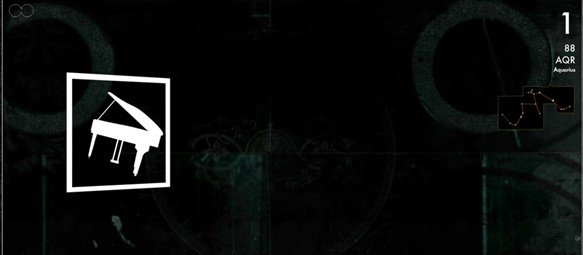
\includegraphics[width=0.6\textwidth]{Fig3[1].jpg}
 \caption{Representação da música na constelação 88 (AQU).}
 \label{fig3}
 \source{\url{http://www.88constellations.net/88.html}.}
\end{figure}

\begin{figure}[htbp]
 \centering
 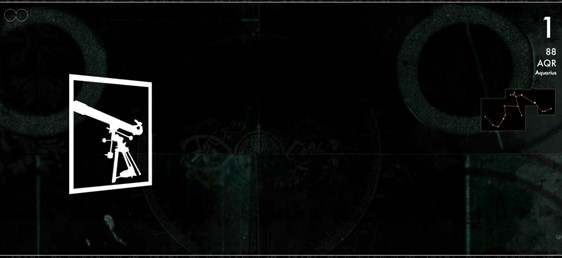
\includegraphics[width=0.6\textwidth]{Fig4[1].jpg}
 \caption{Representação da astronomia na constelação 88 (AQU).}
 \label{fig4}
 \source{\url{http://www.88constellations.net/88.html}.}
\end{figure}

A constelação 88 é introdutória e dela derivam as constelações \emph{Gemini} (GEM), \emph{Psycho} (AQL) e \emph{Twin Towers} (LYR). De maneiras diferentes, todas têm forte presença da dualidade, elemento que perpassa temática e formalmente \emph{88 Constellations}. A constelação \emph{Gemini} (GEM) (\Cref{fig5}) apresenta uma discussão a respeito das complexas relações estabelecidas entre irmãos gêmeos: 

\begin{quote}
Gêmeos são presos na matriz da mesma coisa e da diferença: os mesmos, mas diferentes; diferentes, mas os mesmos. Gêmeos são um paradoxo. São idênticos, mas não simultâneos. Não são um duplo, mas uma coisa que existe duas vezes. Duas coisas que compartilham a mesma aparência, mas que têm existências separadas. Todos nós somos gêmeos. Nós somos idênticos a nós mesmos. Pode-se dizer que nós somos irmãos siameses conectados em todos os lugares. Nós somos ao mesmo tempo o que pensamos de nós mesmos e o que nós pensamos que pensamos de nós mesmos. \cite[n. p., tradução nossa]{clark2010}\footnote{No original: \emph{Twins are caught in the matrix of sameness and difference: Same but different, different but the same. Twins are a paradox. Identical, but not simultaneous. Not a double, but a thing that exists twice. Two things that share appearance but have separate existences. We are all twins. We are identical to ourselves. You can say that we are Siamese twins connected everywhere. We are both things that think of ourselves and the thing we think of we think of ourselves}.}.
\end{quote}

\begin{figure}[htbp]
 \centering
 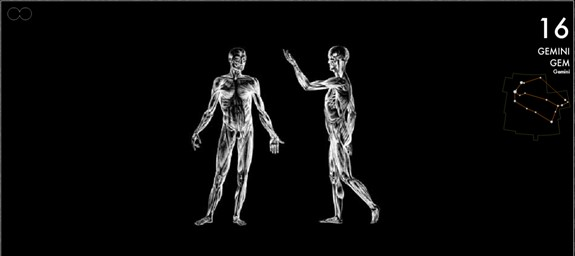
\includegraphics[width=0.6\textwidth]{Fig5[1].jpg}
 \caption{Constelação Gemini (GEM).}
 \label{fig5}
 \source{\url{http://www.88constellations.net/88.html}.}
\end{figure}

Durante a apresentação do texto pelo narrador, há uma fotografia antiga de irmãs gêmeas que, em flashes, trocam de rosto uma com a outra, mudando de posição depois de alguns segundos. Há uma alternância também nas palavras same e different, posicionadas de acordo com a alternância de rostos das gêmeas, conforme representado nas \cref{fig6,fig7}: 

\begin{figure}[htbp]
 \centering
 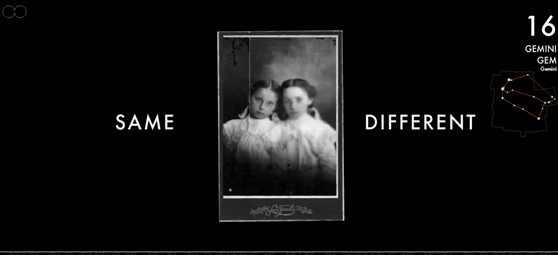
\includegraphics[width=0.6\textwidth]{Fig6[1].jpg}
 \caption{Alternância de rostos das irmãs gêmeas e das palavras \emph{same} e \emph{different}, na constelação Gemini (GEM).}
 \label{fig6}
 \source{\url{http://www.88constellations.net/88.html}.}
\end{figure}

\begin{figure}[htbp]
 \centering
 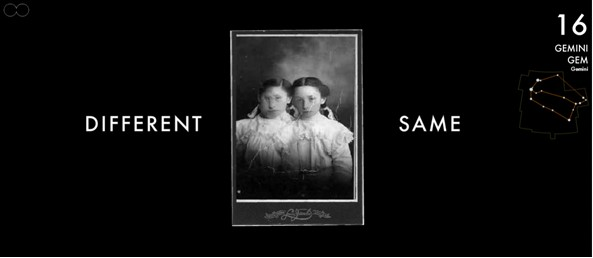
\includegraphics[width=0.6\textwidth]{Fig7[1].jpg}
 \caption{Alternância de rostos das irmãs gêmeas e das palavras \emph{different} e \emph{same}, na constelação Gemini (GEM).}
 \label{fig7}
 \source{\url{http://www.88constellations.net/88.html}.}
\end{figure}

Para além do paradoxo de irmãos gêmeos que, de alguma forma, compartilham sua existência, Clark levanta uma questão que vale para todos os seres humanos: somos sempre duplos, já que temos consciência de nós mesmos e também consciência de que temos consciência de nós mesmos. Essa é uma discussão filosófica central da teoria de Wittgenstein que Clark apresenta por meio de metáforas estruturadas pela confluência de diferentes mídias. 

Se pensarmos que somos todos siameses interconectados, como afirma o narrador, reproduzimos nessas ligações o modelo hipertextual que conecta as constelações no céu e as lexias na obra \emph{88 Constellations for Wittgenstein (to be Played with the Left Hand)}. A dualidade do ser humano – consciência de nós mesmos e consciência dessa consciência – é também evidente na próxima constelação visitada, \emph{Psycho} (AQL), ilustrada na \Cref{fig8}, que leva esse título em razão do filme de Alfred Hitchcock de 1960, conhecido no Brasil como \emph{Psicose}.

\begin{figure}[htbp]
 \centering
 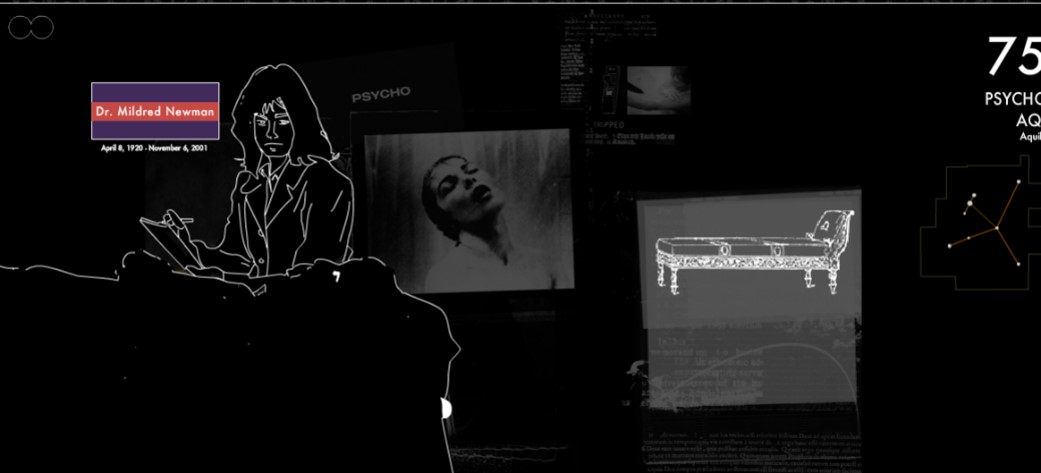
\includegraphics[width=0.6\textwidth]{Fig8[1].jpg}
 \caption{Constelação \emph{Psycho} (AQL).}
 \label{fig8}
 \source{\url{http://www.88constellations.net/88.html}.}
\end{figure}

O filme é uma referência do gênero suspense e compreende uma das cenas mais famosas da história do cinema: o assassinato a facadas da personagem Marion Crane, durante um banho no Hotel Bates. Apesar de trazer algumas curiosidades sobre o filme mundialmente famoso, entre elas que Psicose foi a primeira película a mostrar uma descarga em funcionamento, e que o assassino do filme é baseado no mesmo \emph{serial killer} que inspirou o autor de O silêncio dos inocentes, o narrador de \emph{88 Constellations} incorre nessas digressões para apresentar o caso do ator Anthony Perkins, consagrado pela sua personagem no filme, Norman Bates, proprietário do hotel e assassino. 

A dualidade, nessa constelação, surge de duas formas: em Norman Bates, o personagem que, após assassinar sua própria mãe, apropria-se de sua personalidade e passa a viver uma vida dupla; e no ator que o interpreta, que teve de viver uma vida dupla para fugir dos preconceitos da indústria do cinema à época. Clark apresenta ao leitor a perspectiva da psicanalista de Perkins, a qual precisou analisar uma série de situações que causaram efeitos de dualidade no ator na lida com o público, que por vezes não distinguia o personagem do ator. O foco principal foi no fato de o ator ser homossexual e levar uma vida de aparências para que a indústria do entretenimento não o repelisse. Clark questiona, então: 

\begin{quote}
Se você fosse uma vidente, e não uma psicanalista, veria que Anthony Perkins acabaria tendo que enfrentar essa vida dupla porque ele morreria de AIDS em 12 de setembro de 1992, quase exatamente nove anos antes de sua viúva morrer a bordo do voo 11, quando este colidiu com a Torre Norte do World Trade Center, em 11 de setembro de 2001. Você sabe como o futuro se encaminha, você sabe como a imagem de Perkins sobrevive depois dele. […] Que tipo de psicanálise você oferece? \cite[n. p., tradução nossa]{clark2010}\footnote{No original: If you were a fortune teller, and not a psychoanalyst, you would see that Anthony Perkings would eventually have to confront this double life because he will die of AIDS on September 12th, 1992, almost exactly nine years before his widow would die on board flight 8A11 when it crashes on the north tower of World Trade Center on September 11th, 2001. You know how these things are going to the future, you know how Perkins’ image survives after him. […] What kind of psychoanalysis do you offer?}.
\end{quote}

No início dos anos 1990, morrer em decorrência da AIDS era tomado por grande parte da sociedade e alardeado pela mídia como suposto sinônimo de promiscuidade e preconceituosamente associado à homossexualidade. Anthony Perkins teve, então, ao final da vida, sua intimidade aberta ao público, mas morreu sem revelar detalhes de sua sexualidade. No entanto, a imagem imortalizada de Perkins no imaginário popular foi a de Norman Bates (\Cref{fig9}), replicando os efeitos de duplicidade entre ator e personagem, vida pública e vida privada, Norman Bates e Norma Bates, que essa constelação evoca. 

\begin{figure}[htbp]
 \centering
 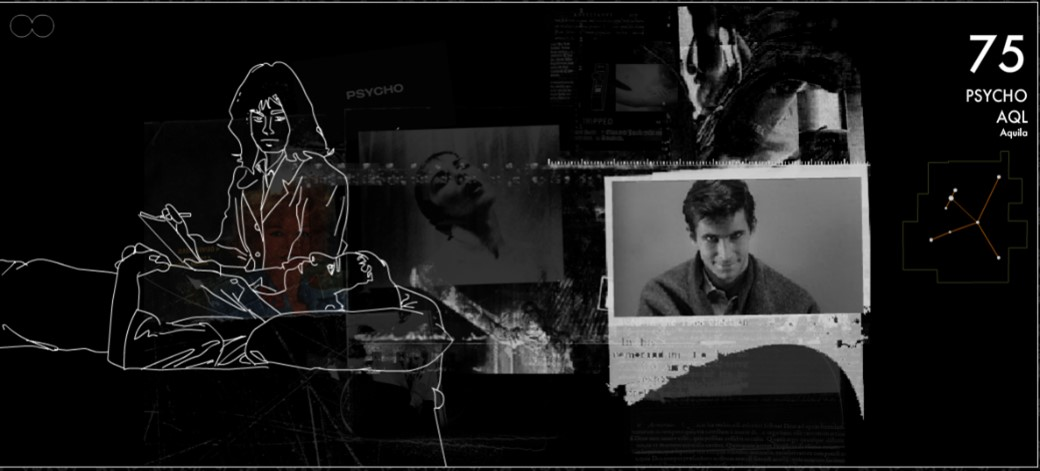
\includegraphics[width=0.6\textwidth]{Fig9[1].jpg}
 \caption{Personagem Norman Bates, interpretada por Anthony Perkins no filme \emph{Psycho} (1960).}
 \label{fig9}
 \source{\url{http://www.88constellations.net/88.html}.}
\end{figure}

O fato de a viúva de Anthony Perkins estar a bordo de um dos aviões que se chocou contra as torres gêmeas no atentado de 2001 leva à conexão com a constelação \emph{Twin Towers} (LYR) (\Cref{fig10}), que apresenta duas imagens, cada uma representando um par de torres gêmeas: Petronia Towers, em Kuala Lumpur, e o World Trade Center, que se encontrava na cidade de Nova Iorque antes do ataque terrorista de 11 de setembro. 

Após o acesso à constelação, há imagens com silhuetas dos dois pares de torres gêmeas, e o leitor tem a opção de clicar em qual desejar. Na silhueta que dá acesso às informações das Petronia Towers, a relação com \emph{88 Constellations} está marcada pelo fato de cada uma das torres ter oito lados (\Cref{fig11}), formando, assim, o número 88, e pelos prédios possuírem 88 andares cada. 

Já o link sob a silhueta de torres gêmeas abre-se para a história da construção do World Trade Center e o impacto negativo causado por sua estética quando da sua inauguração. Apesar de o World Trade Center ser lembrado pelo atentado sofrido em 11 de setembro de 2001, a única menção ao ataque terrorista em \emph{88 Constellations} está relacionada ao fato de que, em 1976, a cena principal do filme \emph{King Kong}, no remake desse ano, foi gravada no World Trade Center, embora a mesma cena, na versão anterior, tivesse sido ambientada no Empire State Building. Após a queda das torres gêmeas, a próxima versão do filme teve de retornar à locação original, como revela o narrador nessa constelação.

\begin{figure}[htbp]
 \centering
 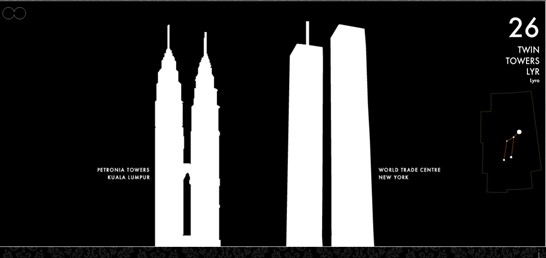
\includegraphics[width=0.6\textwidth]{Fig10[1].jpg}
 \caption{Constelação \emph{Twin Towers} (VEL) com as silhuetas das duas torres gêmeas, Petronia Towers e World Trade Center.}
 \label{fig10}
 \source{\url{http://www.88constellations.net/88.html}.}
\end{figure}

\begin{figure}[htbp]
 \centering
 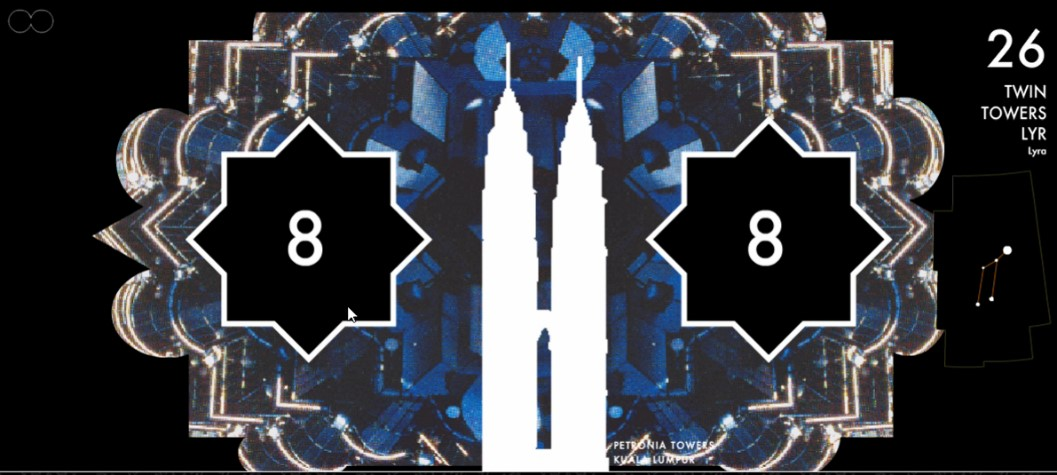
\includegraphics[width=0.6\textwidth]{Fig11[1].jpg}
 \caption{Torres do Petronia Towers, evidenciando a existência de oito lados em cada um dos prédios e a formação do número 88.}
 \label{fig11}
 \source{\url{http://www.88constellations.net/88.html}.}
\end{figure}

Nesse grande labirinto, a característica hipertextual da obra, em que se pode ver a conexão entre diferentes lexias de forma livre, direciona-nos a uma aproximação da metáfora rizomática de \textcite{deleuze1997}. Ao se referirem ao conceito de livro – por nós aplicado a \emph{88 Constellations} como obra ciberliterária –, os autores evidenciam a ideia de conexão e não de unidade monolítica:

\begin{quote}
Não há diferença entre aquilo de que um livro fala e a maneira como é feito. Um livro tampouco tem objeto. Considerado como agenciamento, ele está somente em conexão com outros agenciamentos, em relação com outros corpos sem órgãos. Não se perguntará nunca o que um livro quer dizer, significado ou significante, não se buscará nada compreender num livro, perguntar-se-á com o que ele funciona, em conexão com o que ele faz ou não passar intensidades, em que multiplicidades ele se introduz e metamorfoseia a sua, com que corpos sem órgãos ele faz convergir o seu \cite[p. 11]{deleuze1997}.
\end{quote}

As múltiplas entradas e saídas de \emph{88 Constellations for Wittgenstein (to Be Played with the Left Hand)}, em que se pode navegar de uma constelação a outra e traçar a narrativa no decorrer da leitura, assemelham-se também ao que foi proposto no livro Kafka, por uma literatura menor \cite*{deleuze1977}, no qual Deleuze e Guattari discutem o conceito de rizoma no texto literário. Tal conceito, caro ao pós-estruturalismo francês, marca fortemente uma primeira onda de estudos sobre literatura digital, os quais aplicavam teorias da desconstrução, do rizoma e da morte do autor, entre outras, à análise de hipertextos. Mais trade, porém, tais objetos passaram a ser lidos também à luz dos conceitos dos estudos de mídia, sobretudo aqueles que destacavam as especificidades da literatura digital, conforme apresentado na introdução a este artigo.

Noções de origem, posse ou autoria sobre uma obra literária, colocadas em xeque na teoria rizomática e em outras abordagens pós-estruturalistas, também são vacilantes em \emph{88 Constellations for Wittgenstein (to Be Played with the Left Hand)}. A interpretação de tal obra é sempre aberta ou reatualizada na leitura, pois, de alguma forma, o leitor é também coautor do texto que lê, ao traçar sua própria rota enquanto escolhe os elementos da interface sobre os quais clica. Há um ar de devir no processo de significação da obra, que muda (ou pode mudar) a cada escolha do leitor. 

Entretanto, a obra de Clark não se conforma por completo ao modelo teórico do rizoma, uma vez que ela dispõe de um pivô suportante – o que diferenciava, para \textcite{deleuze1997}, um rizoma de uma raiz. Em \emph{88 Constellations}, há um elemento nuclear tão patente que, no mapa, é representado no centro da tela e de forma emblemática: o cinturão de Orion, que designa o próprio Wittgenstein. Assim, na arquitetura da obra e em sua narrativa, o eixo estruturante é o filósofo. A relação entre as constelações se dá a partir dele e, se ele for suprimido, a estrutura de significação da obra é ceifada. A importância do filósofo para a obra já se faz presente desde o título da obra: ela é para Wittgenstein, raiz, e não rizoma deste universo. 

Outro elemento importante para a conexão entre os fragmentos da obra é a mão, presente no subtítulo da obra \emph{(to Be Played with the Left Hand)} e mencionada reiteradamente de forma mais ou menos aprofundada a depender da constelação. Na próxima seção (\ref{sec3}), será apresentado o segundo percurso de leitura que adotamos, com a imagem da mão como eixo norteador. 

\section{As 88 constelações de Clark: o percurso da mão}\label{sec3}
Há, na vinheta introdutória de 88 Constellations, uma mão esquerda que se movimenta ao lado de um globo em translação. A primeira constelação visitada para este percurso é \emph{Hand} (MEN). Sua imagem inicial é representada pela \Cref{fig12}:  

\begin{figure}[htbp]
 \centering
 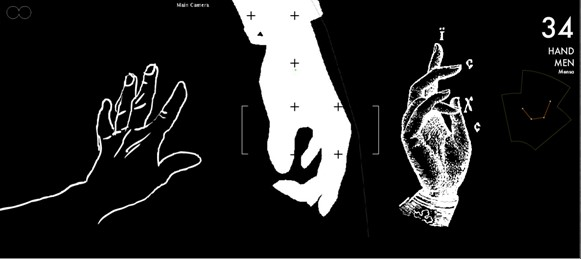
\includegraphics[width=0.6\textwidth]{Fig12[1].jpg}
 \caption{Representações de mãos no início da constelação Hand (MEN).}
 \label{fig12}
 \source{\url{http://www.88constellations.net/88.html}.}
\end{figure}

Ao selecionar a constelação \emph{Hand} (MEN), ouve-se uma narração em off com as seguintes formulações:  

\begin{quote}
Uma mão alcança o mundo. Ela agarra coisas antes que nossa mente o faça. Esta coisa notável, esta mão, este polegar, estes dedos. O número criou a matemática, o mundo digital. Zeros e uns, polegares e dedos [...] tudo e nada. \cite[n. p., tradução nossa]{clark2010}\footnote{No original: \emph{A hand reaches the world. It grasps things before our mind does. This remarkable thing: this hand, this thumb, this finger. The number creates the mathematics, the digital world. Zeros and ones, thumbs and fingers, something and nothing...}}.
\end{quote}

O autor faz referência ao código binário, composto pelos dígitos – do mesmo étimo que dedos e digitais – 0 e 1, responsáveis pelo funcionamento do computador. As imagens que surgem durante o texto do narrador associam os números 0 (nada) e 1 (algo) à forma de uma mão, como ilustrado na \Cref{fig13}. Tal representação do algo (1) e do nada (0) é retomada em outra imagem estilizada da mão humana, conforme verificado na \Cref{fig14}, bem como na grafia das palavras something e nothing, em que a obra brinca com a semelhança gráfica entre as letras I e O e os algarismos 1 e 0.

\begin{figure}[htbp]
 \centering
 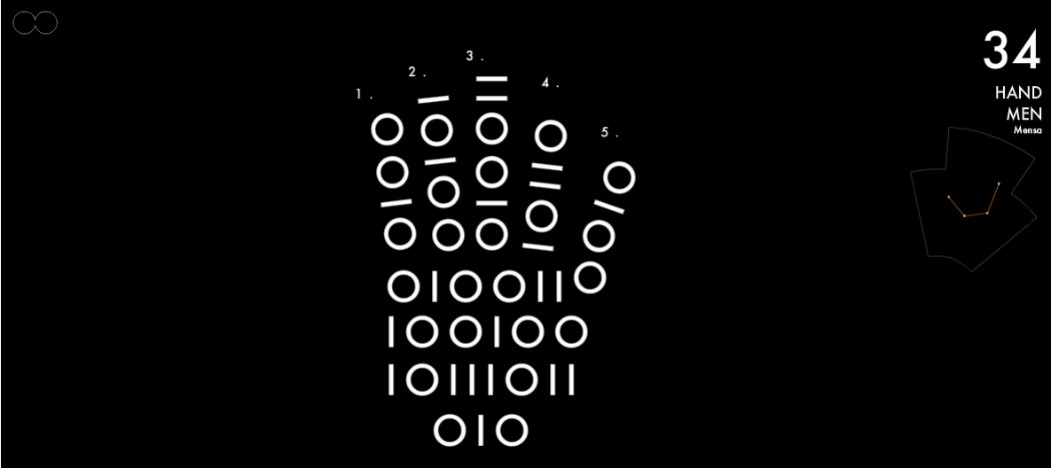
\includegraphics[width=0.6\textwidth]{Fig13[1].jpg}
 \caption{Forma de uma mão constituída por elementos do código binário.}
 \label{fig13}
 \source{\url{http://www.88constellations.net/88.html}.}
\end{figure}

\begin{figure}[htbp]
 \centering
 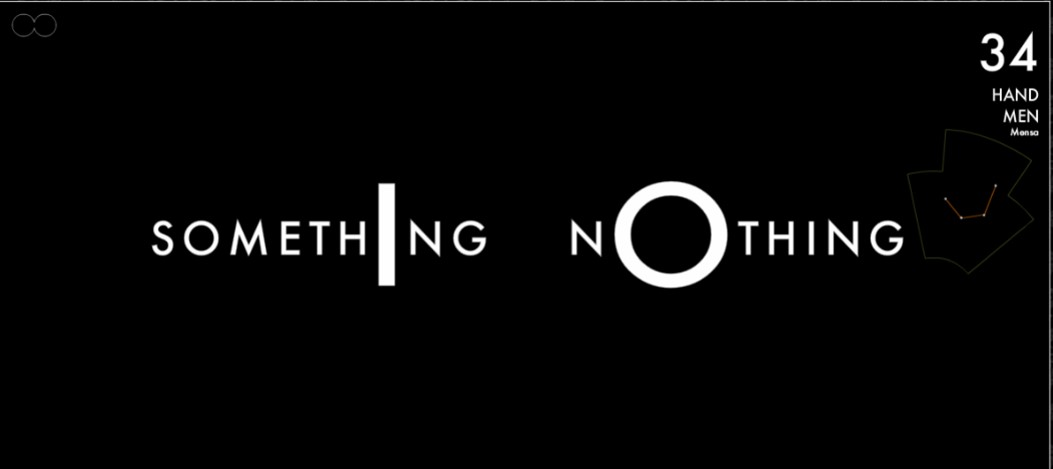
\includegraphics[width=0.6\textwidth]{Fig14[1].jpg}
 \caption{Referência ao código binário nas palavras \emph{something} (algo) e \emph{nothing} (nada).}
 \label{fig14}
 \source{\url{http://www.88constellations.net/88.html}.}
\end{figure}

Mais à frente, é dito na lexia que, quando o homem deixou de usar os membros superiores para se locomover e os pés ficaram responsáveis por essa função, as mãos e seu movimento de pinça tiveram um grande papel para a evolução do ser humano, como na teoria do polegar opositor. É sabido que, quando a humanidade passou a usar as mãos para pegar os objetos, a boca foi isenta dessa função, como parte importante do longo processo evolutivo de desenvolvimento da fala e da linguagem – esta, tema central no projeto filosófico wittgensteiniano.  

Ainda que em proporção menor, evidentemente, também o desenvolvimento do código binário trouxe mudanças significativas para a humanidade, donde se infere a evidente relação entre a linguagem humana e o sistema formado pela boca e pelas mãos.  A era digital alterou o funcionamento do mundo de diversas maneiras, inclusive como a mão é utilizada no dia a dia. Até o século passado, a máquina de escrever exigia o uso das duas mãos igualmente. Desde o lançamento do computador pessoal, passou-se a fazer uso simultâneo de dispositivos como o mouse e o teclado. 

Nesse sentido, cumpre ressaltar que, considerando-se que a maioria da população mundial é destra, empresas de hardware praticamente universalizaram o desenvolvimento de mouses para a mão direita. Alguns sistemas operacionais disponibilizam a função de inverter os botões do mouse para o uso por canhotos, mas o desenvolvimento para uso pela mão direita ainda é a opção padrão. Já os laptops, bastante utilizados hoje, possuem um \emph{touchpad} central, não posicionado ao lado direito da máquina, embora a disposição de seus botões replique o convencionado uso do mouse com a mão direita. Tem-se, então, um “aprisionamento” da mão direita pela máquina operada. Sobre a mão esquerda, \textcite{clark2010} diz, na constelação \emph{Left Hand}: 

\begin{quote}
Por outro lado, a mão esquerda, a mão que foi abandonada na era digital. A mão direita tem trabalho dobrado, pulando do teclado para o mouse. Elas costumavam tocar juntas tão bem ao piano, na máquina de escrever. Elas aprenderam a dançar juntas nas teclas do alfabeto. Mas, agora, na tela do computador, a mão direita é companheira do olho. A mão direita é agora parte do olho. Nossa mente está dividida entre linguagem e música, e nosso corpo e mente foram rasgados pela linguagem. \cite[n. p.]{clark2010}\footnote{No original: \emph{On the other hand, the left hand, the hand that is left, left behind in the digital age. The right hand has double duty, jumping from keyboard to mouse. They used to play together so nicely on the piano, on the typewriter. They learned to dance together on the keys of the alphabet. But now, on the computer screen, the right hand is joining the eye. The right hand is now part of the eye. Observe-se, porém, que o sentido da expressão on the other hand foi perdido na tradução. A expressão teve de ser substituída por “por outro lado”, por não haver correspondente brasileiro que utilize a palavra “mão” para indicar a mesma ideia. O jogo de palavras entre left (deixada) e left (esquerda) também foi perdido na tradução, mas precisa ser considerado em uma análise imanente da obra de David Clark.}}.
\end{quote}

\begin{figure}[htbp]
 \centering
 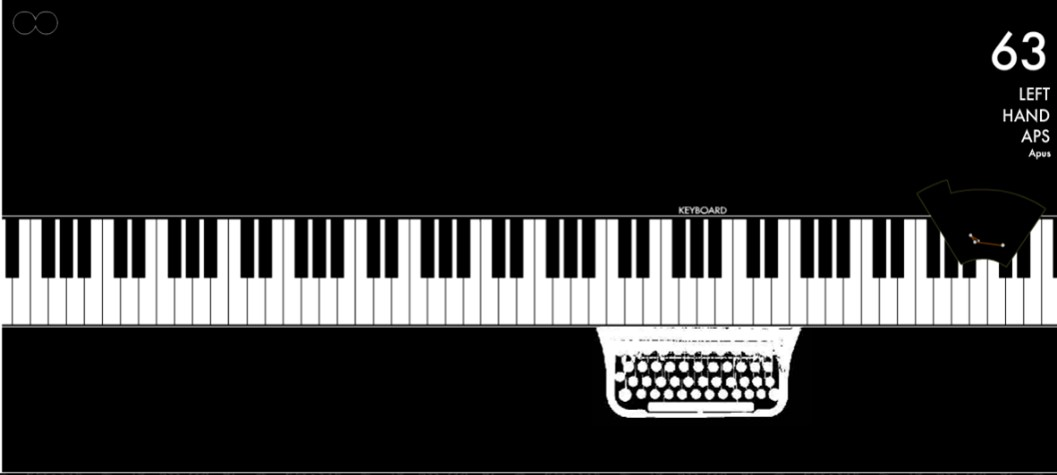
\includegraphics[width=0.6\textwidth]{Fig15[1].jpg}
 \caption{Representação de teclados de piano e de máquina de escrever na constelação \emph{Left Hand}.}
 \label{fig15}
 \source{\url{http://www.88constellations.net/88.html}.}
\end{figure}

Por sua vez, o irmão de Ludwig Wittgenstein, Paul, perdeu uma de suas mãos, limitando-se ao uso da mão esquerda, fato este tematizado na constelação Paul Wittgenstein (PAV) (\Cref{fig16}). 

\begin{figure}[htbp]
 \centering
 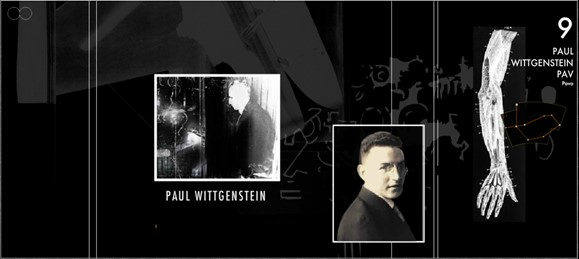
\includegraphics[width=0.6\textwidth]{Fig16[1].jpg}
 \caption{Paul Wittgenstein, irmão de Ludwig Wittgenstein.}
 \label{fig16}
 \source{\url{http://www.88constellations.net/88.html}.}
\end{figure}

O primeiro frame dessa constelação apresenta trecho em vídeo de uma série intitulada \emph{M*A*S*H*}, dos anos 1970, em que um dos personagens conta a outro como se deu a composição do concerto de Maurice Ravel para a mão esquerda, levando ao nome de Paul Wittgenstein (\Cref{fig17}).

\begin{figure}[htbp]
 \centering
 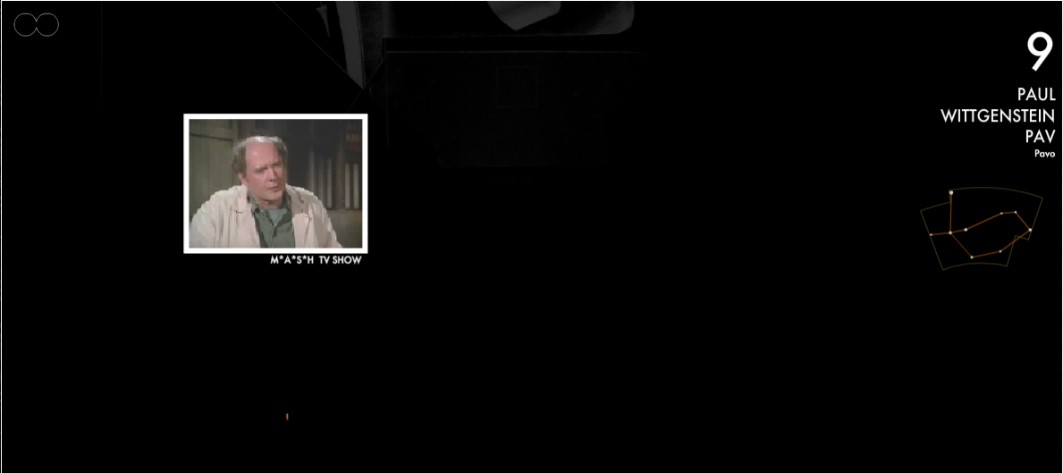
\includegraphics[width=0.6\textwidth]{Fig17[1].jpg}
 \caption{Exibição de um trecho de programa de TV que cita Ravel e Paul Wittgenstein.}
 \label{fig17}
 \source{\url{http://www.88constellations.net/88.html}.}
\end{figure}

Para que continuasse a tocar piano, Paul Wittgenstein encomendou a alguns compositores da época peças para que pudesse executar apenas com a mão esquerda. David Clark, ao utilizar no título de sua obra a expressão \emph{to be Played with the Left Hand}, referia-se tanto ao irmão do filósofo quanto ao fato de, em \emph{88 Constellations for Wittgenstein}, alguns comandos terem sido programados para que, quando o leitor utilizasse o teclado durante a leitura (já que a mão direita estaria realizando o trabalho de selecionar, com o mouse, as constelações de sua preferência), fossem emitidos sons e surgissem imagens na tela durante a exibição base, aquela mostrada apenas por seleção. Assim, o leitor joga e toca com a mão esquerda, o que replica, para o nível da interação física com o hardware e a interface digital, semas relacionados ao duplo e à mão, recuperados ao longo do exercício de \emph{close reading} a partir de rotas temáticas no hipertexto, conforme descrito neste artigo. 

Arrematando este exercício de leitura de \emph{88 Constellations}, em sua materialidade digital hipertextual e alguns dos principais temas que a obra enseja, podemos ainda retomar uma célebre fala do escritor português Gonçalo M. Tavares, que, em entrevista a Cassio Hissa, faz uma analogia ao uso da mão esquerda, a partir de uma citação de Walter Benjamin: 

\begin{quote}
Gosto dessa ideia: a de tentar produzir a partir de metodologias que nos são estranhas, e com isso, nos surpreender. Há uma ideia que valorizo muito, de Walter Benjamin (1892-1940): numa frase: os golpes decisivos serão desferidos com a mão esquerda. [...] Eu acredito que, provavelmente, os resultados mais criativos, mais decisivos – eu estou agora, nesse momento, a pensar nisso – serão produzidos a partir de uma metodologia à esquerda. \cite[p. 127]{tavares2011}.
\end{quote}

Se levarmos em consideração que, ainda nos dias de hoje, o livro de papel configura o objeto de maior valor e o suporte mais frequente na cultura literária, poderíamos dizer que, segundo o pensamento de Tavares, a literatura impressa, em sua forma convencional, seria produzida a partir de uma metodologia à direita. Por outro lado, a ciberliteratura, ao se valer de expedientes distintos dos já institucionalizados, é, portanto, estranha, ou sinistra – escrita, afinal, com a mão esquerda, como bem nos mostra esta análise detalhada do romance hipertextual de David Clark. 

\section{Considerações finais}
Este artigo apresentou os percursos temáticos da imagem do duplo e da mão, selecionados entre os outros percursos possíveis dentro de \emph{88 Constellations for Wittgenstein (to Be Played with the Left Hand)}. A escolha de tais temas se deu durante uma leitura analítica do hipertexto em busca de significados recorrentes na rede interpretativa que se nos apresentava. Para recomposição dos fios interpretativos que os recorrentes semas constroem por meio das escolhas dos autores do presente artigo (entre tantas outras escolhas possíveis), optamos por uma análise imanente, centrada em operações de \emph{close reading}. Além dos ganhos que tal metodologia aporta em termos da dissecação de particularidades da obra, ressalte-se um segundo benefício que ela acarreta no caso de uma produção artística como \emph{88 Constellations}, a qual carece de documentação por meio de textos, capturas de tela etc. na medida em que sua materialidade digital, programada em Flash, é hoje inacessível pelos mais populares navegadores de Internet.

Na obra analisada neste artigo, bem como em outras de literatura digital, a leitura se dá por procedimentos interativos e hipertextuais, por meio dos quais as partes se ligam como pontos em um jogo, por movimentos entre duplos, conexões e replicações, traçadas com a mão esquerda, fato já indicado no subtítulo com a palavra left. 

Quanto ao que conota o termo “esquerda”, cumpre lembrar que o canhoto assume vários sentidos, de obliquidade a diferença no senso comum, colocando-se em oposição ao lado direito. Então, seja por referências duplicadas e deslizantes à vida de Wittgenstein e de sua família, que outras constelações da obra evocam (evidente no episódio em que o irmão perde a mão e encomenda um concerto para a mão esquerda para Maurice Ravel, que Paul Wittgenstein tocava ao piano), a obra de Clark se mostra um ludo para canhotos. Como labilidade interpretativa, o leitor avança pelo texto apenas à esquerda, multilinear e obliquamente – e não à direita, de modo linear ou reto –, entrelaçando signos como estrelas para recompor lampejos de Wittgenstein. 

Foi possível notar, dentro de ambos os percursos escolhidos nesta leitura, uma vasta gama de informações de períodos históricos diferentes, de cunho histórico, filosófico e científico. Tal fato aponta que, dentro de suas especificidades, a ciberliteratura pode também ser uma ferramenta para difusão de saberes das mais diversas áreas de conhecimento, tema a ser investigado em desdobramentos futuros desta pesquisa. 

A obra analisada neste artigo, \emph{88 Constellations for Wittgenstein (to be Played with the Left Hand)}, encerra aquilo que é necessário para contar a história de Ludwig Wittgenstein e faz bem seu trabalho: proporciona a construção de saberes, a Mathesis que Roland \textcite{barthes2004} defende como sendo uma das três funções da literatura. Por essa característica, 88 Constellations, assim como outras obras da ciberliteratura, pode ser aplicada ao ensino em diversas áreas de conhecimento, como filosofia, língua estrangeira, história e geografia. Navegar por entre as constelações em \emph{88 Constellations} possibilita que se conheçam, primariamente, alguns dos conceitos fundamentais do pensamento de Wittgenstein, que aprofundou os estudos da linguagem na filosofia. Ademais, ressaltando a dimensão de inespecificidade \cite{garramuno2009} cara a um romance hipertextual, tem-se contato com diversas manifestações artísticas, como artes plásticas, música, cinema e fotografia; conhecem-se fatos históricos de alcance mundial; reflete-se de forma lúdica e poética sobre questões filosóficas e sobre problemas socioeconômicos de interesse geral. 

\emph{88 Constellations for Wittgenstein (to be played with the left hand)} apresenta, além dos temas tratados neste artigo, algumas outras características que podem indicar caminhos para pesquisas futuras: como se dá a presença de importantes obras de Wittgenstein, como o Tractatus Logico-Philosophicus e Investigações Filosóficas; temas como a homossexualidade, a guerra, a economia e o cinema; e a oncstituição multimodal da obra, com destaque para os signos audiovisuais. 

Um dos principais desafios para a escrita deste trabalho está no fato de que \emph{88 Constellations} é uma obra hipertextual, não linear, não mais disponível para navegação em navegadores de Internet populares após a obsolescência do Flash, além de ser composta por signos sonoros, visuais e animações, o que demandou um trabalho de gravação e transcrição de textos, além do uso de imagens para explicar como funcionam as constelações. Foi preciso, assim, burlar o sistema de leitura hipertextual e multimodal da obra para que ela se enquadrasse em um artigo acadêmico sobretudo linear e precipuamente verbal.

A ciberliteratura, por suas características inerentes, difere da literatura convencional, impressa, para além de uma simples mudança de suporte. Vídeo, áudio, mobilidade dos blocos de textos, geração de textos a partir de programação de computadores, plasticidade das narrativas: quase todas essas características são impossíveis de serem contempladas – ou só o são de maneira muito inicial – pela literatura impressa. Não se trata de dizer que uma literatura é melhor que outra, mas que são diferentes e que devem ser estudadas de formas diferentes, não hierarquizadas. 



\printbibliography\label{sec-bib}
% if the text is not in Portuguese, it might be necessary to use the code below instead to print the correct ABNT abbreviations [s.n.], [s.l.]
%\begin{portuguese}
%\printbibliography[title={Bibliography}]
%\end{portuguese}


%full list: conceptualization,datacuration,formalanalysis,funding,investigation,methodology,projadm,resources,software,supervision,validation,visualization,writing,review
\begin{contributors}[sec-contributors]
\authorcontribution{Alice Garcia da Silveira}[conceptualization,formalanalysis,investigation,writing,review]
\authorcontribution{Vinícius Carvalho Pereira}[methodology,formalanalysis,investigation,review]
\end{contributors}

\end{document}